% mirko.rahn@itwm.fraunhofer.de

\documentclass[a4paper,12pt]{article}

%\usepackage{tikz}\usetikzlibrary{automata,arrows,snakes,shapes}
\usepackage{amssymb}
\usepackage{amsmath}
\usepackage{ngerman}
\usepackage[latin1]{inputenc}
\usepackage[T1]{fontenc}
\usepackage{microtype}
\usepackage{fixltx2e}
\usepackage{tocloft}
\usepackage{ifthen}
\usepackage[nosepfour]{numprint}
\usepackage{url}
%\usepackage{zref-perpage}
\usepackage{index}
\usepackage{fancyhdr}
\usepackage{booktabs}
\usepackage{moreverb}
%\usepackage{citeref}
\usepackage{xspace}
\usepackage{mparhack}
\usepackage{graphicx}

\begin{document}

\title{Editor f"ur die Fraunhofer Parallel Programming Platform}

\author{Mirko Rahn}

\maketitle

\begin{abstract}
  Im Rahmen des MWARE MAVO produziert das ITWM eine neuartige Platform
  zur schnellen grafischen Entwicklung und effizienter Ausf"uhrung
  paralleler Programme auf HPC Systemen.

  Wir stellen die Anforderungen an und Vorstellungen "uber den
  grafischen Editor dar.
\end{abstract}

\section{Die Plattform}
\subsection{"Uberblick}
Wesentliche Idee ist die Trennung von Koordinierungsprache und
Programmiersprache oder besser Berechnungssprache. Auf der Ebene der
Berechnungssprache sprechen wir "uber Module, die Daten konkret
bearbeiten, "uber Algorithmen. Diese Module wollen und sollen sich
aber nicht k"ummern um zum Beispiel das Herbeischaffen der
Eingabedaten, das Speichern oder Weiterleiten der Ausgabedaten. Das
sind Aufgaben, die auf der Ebene der Koordinierungssprache erledigt
werden. Ebenfalls zur Koordinierung geh"oren (automatische)
Parallelisierung, (automatische) Balancierung der Last, (automatische)
Fehlertoleranz, "Uberwachung des Systems, \ldots \cite{gelernter}

\begin{figure}\label{fig:arch}
\begin{center}
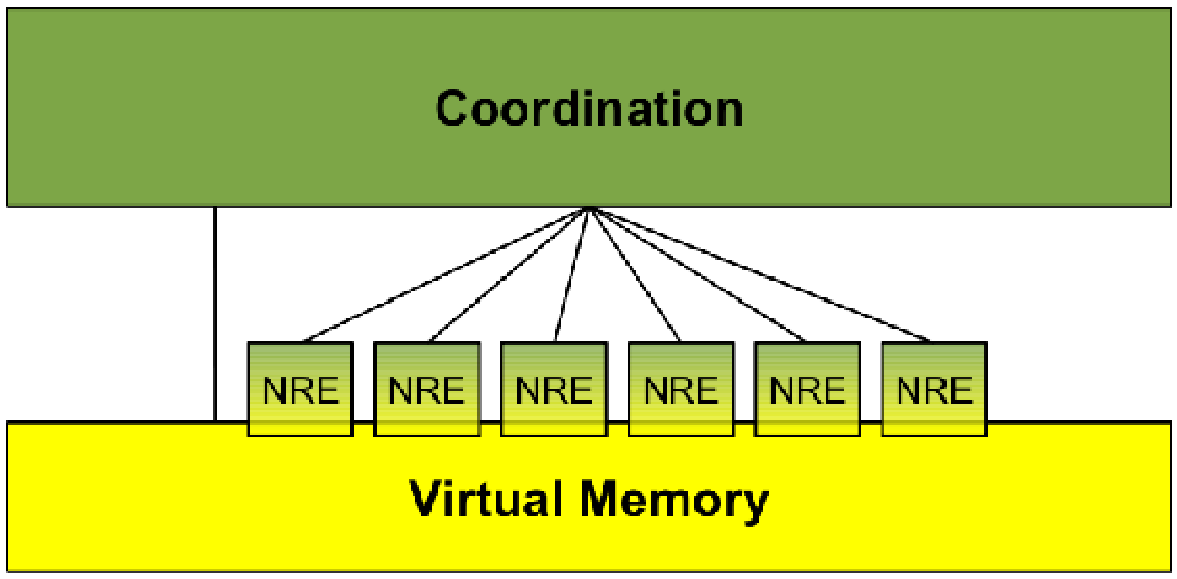
\includegraphics[width=0.8\textwidth]{architecture.pdf}
\end{center}
\caption{Architektur der Plattform}
\end{figure}

\subsection{Definition des Austauschformats}

\section{Der Editor}
\subsection{Level 1: Petri-Netz Editor}
\subsection{Level 2: Editor f"ur Dom"ananwender}
\subsection{Level 3: Exploratives Entwickeln}

\section{Der Monitor}

\renewcommand{\bibname}{Literatur}
\begin{thebibliography}{\quad}

\bibitem{gelernter}D.~Gelernter, N.~Carriero. \emph{Integration or
    Separation.} Communications of the ACM 35(2):97--107, 1992.

\end{thebibliography}

\end{document}